\documentclass[11pt,a4paper]{article}

%\usepackage{pdfsync} %% for pdfview (good PDF viewer for the Mac)
%\usepackage[active]{srcltx} %% for xdvi

\usepackage{verbatim}
\usepackage{amsmath}
\usepackage{graphicx}
\usepackage{parskip}
%\usepackage{epsfig}
\usepackage{url}
\usepackage[colorlinks=true]{hyperref}
\usepackage{listings}
\usepackage{color}
\usepackage{cite}
\usepackage[numbers]{natbib}

\usepackage{geometry}
\geometry{textwidth=38em,textheight=44\baselineskip}

\newcommand{\mycomment}[3]{{\ignorespaces\sffamily[~#1~(#2): #3~]}}
\renewcommand{\mycomment}[3]{\ignorespaces\relax}

\definecolor{Brown}{cmyk}{0,0.81,1,0.60}
\definecolor{OliveGreen}{cmyk}{0.64,0,0.95,0.40}
\definecolor{CadetBlue}{cmyk}{0.82,0.77,0.13,.4}
\definecolor{lightlightgray}{gray}{0.9}

\lstset{
%language=Java,                             % Code langugage
basicstyle=\ttfamily \small,                   % Code font, Examples: \footnotesize, \ttfamily
keywordstyle=\color{CadetBlue},        % Keywords font ('*' = uppercase)
commentstyle=\color{OliveGreen},              % Comments font
numbers=left,                           % Line nums position
%numberstyle=\tiny,                      % Line-numbers fonts
%stepnumber=1,                           % Step between two line-numbers
numbersep=5pt,                          % How far are line-numbers from code
%backgroundcolor=\color{lightlightgray}, % Choose background color
%frame=none,                             % A frame around the code
tabsize=4,                              % Default tab size
%captionpos=b,                           % Caption-position = bottom
%breaklines=true,                        % Automatic line breaking?
%breakatwhitespace=false,                % Automatic breaks only at whitespace?
showspaces=false,                       % Dont make spaces visible
showtabs=false,                         % Dont make tabls visible
showstringspaces=false,
%columns=flexible,                       % Column format
morecomment=[l]{//},
morekeywords={social media, event detection, sentiment analysis, preference learning}
}

%double line
%\linespread{2}

%\COMMENT begins comment
\long\def\COMMENT#1\ENDCOMMENT{\message{(Commented text...)}\par}

%% Check if pdflatex is running
\ifx\pdfoutput\undefined\def\pdfoutput{0}\fi

% Good KR language is notationally efficacious

%\bibliographystyle{alpha}
%\pagestyle{empty}
\begin{document}
\title{\bf A Survey on Using Social Media as a Sensor \\
\large PhD Qualification Exam Report, Summer 2015}
\author{
 \href{http://web.engr.oregonstate.edu/~imanz/}{Zahra Iman} (\texttt{imanz@onid.oregonstate.com}) \\
Oregon State University
}
\date{}

\maketitle

\vspace{-5mm}

\begin{abstract}

\end{abstract}

\vspace{-3mm}

\setcounter{tocdepth}{3}
\tableofcontents

%\newpage
%\vfill

\section{Introduction}

Sensors are devices used for measuring some aspect of an environment and converting it into continuous or discrete value for use in information or control systems. For example, thermocouple as a sensor senses the temperature and converts it to continuous output voltage or a fire detector outputs a boolean value as a result of sensing smoke. Expanding on this definition, social media can be used as a sensor to detect important news e.g., death of Michael Jackson, real-time events e.g., earthquake or epidemics, sentiments and opinions e.g., people's political alignment towards political debates, preferences and traits e.g., stock market prediction or purchase behavior prediction.

However, due to the complexity of information in social media, designing sensors to detect specific phenomena requires highly specialized research to extract targeted information. Designing methodologies and extracting features that are robust to highly dynamic changes in social media, with various forms of expression e.g., informal, short, unstructured texts, written by individuals from different educational levels, and with large volumes of extraneous material mixed in is a difficult task in need of extensive research. 

This paper surveys existing work to explore social media as a sensor, methodology and features developed. This paper concludes by examining open areas for future research.
%This sensory information provides details about various situations, users and their environment across locations and time \cite{rosi}. At the macro level, meaningful news, events, incidents, and health epidemics can be detected as the output. This is done by detecting sensory information from users such as posts, tweets, etc. 
%In this survey, we focus on different aspects of using social media as a sensor. In order to provide more perceptible and practical applications of this concept, use cases of social media sensors are introduced in the first part. These use cases include extraction of events such as celebrity concerts, sentiments such as political sentiment extraction, and preferences such as predicting purchase behaviors from social media. In the second part, the theory supporting each use case is provided.

\section{Use Cases of Social Media Sensor}
\label{usecases}

This section provides existing research on the use of social media as a sensor for three major use cases of events, sentiment, and preference. This information is important for different target users such as government agencies, traffic incident management departments, marketing companies, and individuals.

\subsection{Events}

A social media event can be defined as an occurrence at a certain time interval and geographical region. It can be planned or unexpected e.g, concert vs. death of a celebrity, man-made or natural e.g., parade vs. earthquake, local or global e.g., concert vs. World Peace Day. Events can further be categorized based on their target users, including individuals, government agencies concerned about natural disasters and health epidemics, marketing companies, and news websites. 

Historically, event detection has been studied extensively in text mining, NLP, and IR to find events from conventional media sources such as news streams \citet{yang}. With the growth of social media sites such as Facebook, Twitter and other microblogs, social media sites have become known as powerful communication tools for sharing and exchanging information about such events. However, event detection on social media sites is more challenging due to features such as unstructured and informal text, highly length restricted, generated by novice reporters compared to journalism-trained news editors.%, and generated in real time in many cases. 

Nevertheless, it is important to investigate event detection in social media because in comparison to traditional news blogs, social media has faster response time to events and time is money (marketing), lives (disasters), or simply relevance (new).

To see how different use cases address the aforementioned technical difficulties, we focus on the three highly studied types of event detections:
\begin{itemize}
\item Trending Topic Detection
\item Natural Disaster Detection
\item Health Epidemic Detection
\end{itemize}

In the next section, we summarize the results of trending topic detection research.

\subsubsection{Trending Topic Detection}

Trends i.e. emerging topics are typically driven by emerging events, breaking news and general topics such as death of celebrities, festivals, and sporting events that attract the attention of a large fraction of Twitter users \cite{mathioudakis}. Real-time detection of events which are hypothesized to be trendy is thus of high value for  news reporters and analysts. 

The following works on detecting trending topics use bursts as the indicator of events, where a burst is defined as a sudden change in posting rates of some keywords, hashtags, etc. However, they can be divided into multiple categories based on how they use bursts to extract the event. 

\textbf{Clustering-based Methods} This category of works focus on the hypothesis that trends are topical and topics are defined by collection of relevant content, hence trends can be detected by clustering posts.
\begin{itemize}
\item \textbf{Threads of tweets} \citet{petrovic} tried to detect novel events from streams of Twitter posts by forming threads of similar tweets. The minimum similarity distance to an existing tweet represents novelty score of the tweet. Similarity threshold for assigning tweets to threads controls size of threads. The fastest growing thread in each time interval indicated the news of the event spreading and are outputted as new events. 
\item \textbf{Wavelet analysis} \citet{wangLee} applied wavelet analysis to individual words on the frequency based raw signals of the words and identified events by grouping a set of words with similar burst patterns.
%Compared with DFT, wavelet transformation has more desirable features. Wavelet refers to a quickly varnishing oscillating function [5, 9]. Unlike the sine and cosine used in the DFT, which are localized in frequency but extend infinitely in time, wavelets are localized in both time and frequency domain. Therefore, wavelet transformation is able to provide precise measurements about when and to what extent bursts take place in the signal. 
\end{itemize}

\textbf{Term-based Methods} The second category of works focus on the hypothesis that topics can be detected by focusing on temporal patterns of terms/keywords independent of contents of documents.
\begin{itemize}
\item \textbf{Keyword-burst} \citet{mathioudakis} detected events by focusing on bursts of keywords whereas \citet{cuiZhang} used different hashtag properties to this purpose. \citet{zhaoSports} and \citet{nichols} also tried to use bursts in keywords, but they monitored specific keywords related to sports game in order to detect important NFL games or important moments within the game.
\end{itemize}
\textbf{Term-based Methods} The third category of works focus on detecting trending topics by measuring trendiness factor based on user-defined criteria.
\begin{itemize}
\item \textbf{Location-dependent} Emphasizing location, \citet{albakour} and \citet{sakakiDrive} detected local events based on either user query, user location, or both. \citeauthor{albakour} employed contents of the tweets and volume of microblogging activite for locating events in a local area and ranked tweets on the level of topical relevancy to user query resulting in ranked list of local events. \citeauthor{sakakiDrive} used classification approach for detecting driving events at a local area by using dependency of words to search query, context (words before or after a search query), position of a search query in a tweet, time expression in a tweet, and word features (all words in the tweet) as features. %Results showed that their system can collect tweets referring to heavy traffic from Twitter with 87\% precision and could extract location information from those tweets with 85\% precision.
\item \textbf{Structure-based} \citet{budak} incorporated network topology in order to find trending topics. They defined trendiness of a topic based on two notions, either by the number of connected pairs of users discussing it, or by scoring a topic based on the number of unrelated people interested in it. 
\end{itemize}

\subsubsection{Natural Disaster Detection}

In case of disasters, users will tweet about the disaster within seconds of its happening \footnote{http://mashable.com/2009/08/12/japan-earthquake/}. Using this information, disasters can be detected almost in real time from social media and responded to by government agencies such as U.S. FEMA (Federal Emergency Management Agency), local first responders, news websites, and individuals. The goal of works targeting disastrous events on Twitter can be divided into the two following categories:

\textbf{Predictive studies on disaster} \label{FP} \citet{sandy} studied the network of users and focused on choosing the best groups of users in order to achieve lead-times i.e. faster detection of disastrous event (following the concept of "friendship paradox"\footnote{On average, most people have fewer friends than their friends have}). On the other hand, \citet{sakakiEq2} used SVM classifier for detecting earthquake and employed location estimation method such as Kalman Filtering for localizing it. \citeauthor{sakakiEq2} extracted statistical features e.g., the number and position of words in a tweet, keyword features and word context features. These studies investigated the real-time nature of Twitter and provided promising results.
%introduced in a seminal work by \citet{feld}, showing that "your friends have more friends than you do"

\textbf{Descriptive studies on disaster} Related works discuss the behavior of Twitter users during crisis \cite{vieweg, cheong, starbird} but do not address exploiting detection of crisis events. They investigated the use of social media during crisis in order to identify information propagation properties, social behavior of users e.g. retweeting behavior, information contributing to situational awareness, and active players in communicating information. However, this behavioral information could be exploited in development of sensors.

\subsubsection{Health Epidemic Detection}

A disease outbreak can rapidly infect great numbers of people and expand to broad areas involving several countries such as Ebola \footnote{http://www.cdc.gov/vhf/ebola/outbreaks/index.html}. It is very important to identify the infected sources as early as possible and control the spread of epidemics by incubating infected individuals \cite{eubank,cdcEpidemic}. Target users of this event detection include government agencies such as the CDC (Centers for Disease Control and Prevention), news websites, and individuals.
%Similar to the previous categories, social media can play an important role in this regard. By taking advantage of large numbers of social sensors in the social media, traces of infection can be found  and contagious spread  of information in a global-scale can be modeled. The target users of these type of event detection and identification include government agencies such as the CDC (Centers for Disease Control and Prevention), news websites and individuals.

The purpose of these works was early detection of outbreaks using tweets. Researchers used content-based method and/or structure-based methods outlined as follows:

\textbf{Content-based methods} \citet{culotta} and \citet{aramaki} both tried to identify influenza-related tweets and find correlations of these tweets to CDC statistics.  Both works extracted bag-of-words as features. As for methodology, the former used single and multiple linear regression showing that multiple linear regression works better, while the latter employed SVM. Results showed high correlation of their estimation of influenza in early stages with values from U.S CDC and Japan's Infection Disease Surveillance Center.

\textbf{Structure-based method} In contrast to previous methods, \citet{garcia} focused on a structure-related technique and developed a model for contagious information diffusion in a social network. They provided a method for choosing sensor groups from friends of random sets of users to find more central individuals in order to enforce early detection.

\textbf{Hybrid method} \citet{sadilek} exploited both content and structure information. They employed a semi-supervised approach to learn a robust SVM classifier by training two classifiers on a labeled set and then applying them to non-labeled tweets . This enabled them to model the interplay of social activity, human mobility, and the spread of infectious disease in a large real-world population. Further, \citeauthor{sadelik} identified sick individuals from the content of online communication. %we study the roles that social ties and interactions between specific individuals play in the progress of a contagion

%Monitoring online data with the purpose of advance warning and improved detection of epidemics has been the focus of attention in recent research \cite{garcia, culotta}. \citet{garcia} developed a model of contagious information diffusion in a social network and provided a method for early detection. The method relies on the same concept of "friendship paradox" \cite{feld} used by \citet{feld} in the Hurrican Sandy case. Following the same concept, choosing sensor groups as friends of a random set of users enabled them to find more central individuals. This, was helpful in detecting contagious diseases before outbreaks occurred. 

%Following the same goal of rapid response to health epidemics, \citet{culotta} identified influenza-related tweets in order to study the possible correlations with CDC statistics. They collected 500,000 tweets over 10 weeks by choosing a set of keywords. They investigated several regression methods to predict rates of influenza-like illnesses in a population based on frequency of messages containing certain keywords. \citet{aramaki} also tried to detect influenza epidemics in Twitter. However, they used SVM classifier in order to collect tweets mentioning actual influenza patients. Results showed high correlation of their estimation of influenza in early stages with gold standard values from Japan's Infection Disease Surveillance Center (IDSC) data.% which gathers influenza patient data from 5,000 clinics and releases summary reports.

\subsection{Sentiments and Opinions}
\label{sentiment_section}

Sentiment analysis, also known as opinion mining, is defined as analysis of text based on expressed sentiments by users. Users share their opinions about products, political matters, the stock market, and pharmaceuticals \footnote{pharmacological science relating to the collection, detection, assessment, monitoring, and prevention of adverse effects of pharmaceutical products}. Marketing companies, government agencies, and individuals are concerned with what users think about them/their products. The goal here is to learn the model of users' sentiment toward these matters. To this purpose, different classification and statistical methods are used that are mentioned in the following sections.


\subsubsection{Types of Sentiment Analysis}

Two major aspects of sentiment analysis are the following:

\textbf{Subjective vs. Objective sentiment} At the top level of analysis, sentiment can be classified as subjective or objective \cite{liu09}. Subjective text indicates a writer's opinion or emotional state with respect to some topic e.g., "it's an excellent phone", while objective text indicates a desirable or undesirable condition e.g., "it is broken". %For example, \citet{kouloumpis} classified tweets in order to learn the polarity of phrases while \citet{pakpar} classified text as objective or subjective. Then, they identified the polarity of subjective texts. Both methods use n-grams, POS-tags features. However, \citet{kouloumpis} uses microblogging features such as presence of intensifiers, positive/negative/neutral emoticons and abbreviations as well. Following, we provide more targeted research for various applications of sentiment analysis. 

\textbf{Simple vs. Complex sentiment } Simple sentiment shows whether a text's attitude is positive or negative. Complex sentiment involves the sentimental reaction of the human to various words across different factors, such as measuring the scale of positivity/negativity, potency, oriented activity, receptivity, aggressiveness, novelty, and tension and will be discussed in the applications of sentiment analysis.

Regardless of the features and sentiment type, sentiment analysis in social media has different application which are discussed in more detail in the following sections. 

\subsubsection{Framework of Sentiment Analysis}

Methods used in sentiment analysis included:

\begin{itemize}
\item Classification e.g., SVM, NB, Maximum Entropy, Neural Network
\item Manual Coding and Concept Extraction
\item Simple Statistical Methods
\item Textual Analysis Softwares
\end{itemize}

$
Methods\left\{\begin{matrix}
Classification\ e.g.\ SVM,\ NB,\ Maximum\ Entropy,\ Neural\ Network\\ 
Manual\ Coding\ and\ Concept\ Extraction\\ 
Simple\ Statistical\ Methods\\ 
Textual\ Analysis\ Softwares
\end{matrix}\right.
$

$
Features\left\{\begin{matrix}
n-grams\ e.g.,\ uni-gram,\ bigram,\ and\ trigram\\ 
POS-Tags\\ 
Negations\\ 
Colocation\ and\ Position\ of\ words\\
Semantic\ features\ e.g.,\ extracting\ concept\ from\ medical\ dictionary
\end{matrix}\right.
$
\subsubsection{Applications of Sentiment Analysis}

%The second category of sentiment analysis research includes different applications of sentiment analysis on social media. In this regard, use of social media as a sensor is investigated with respect to different goals. For example analyzing social data for extraction of political sentiment can provide government agencies, political parties, and individuals with a broader view on people's ideas about certain politicians or political events. Therefore, each application provides different viewpoints on extracted sentiments and targets distinct groups as their main users. 

\textbf{Political Applications}
Social media has been extensively used during political events. For example, analysts attribute Obama's victory to the strength of his social-networking strategy and use of social media such as mybarackobama.com, or MyBO \cite{tumasjan} which shows the extent and influence social networking holds during political debates and events.

Researchers have studied social media in order to either investigate and evaluate the relationship of online political sentiment to offline political landscape \cite{tumasjan, bakliwal, oconnorPolitics, wangCan} or to see if online political sentiment can be predictive of actual election results \cite{mejova, bermingham}. Methodologies used for these purposes include using textual analysis software (LIWC \cite{LWIC07}) \cite{tumasjan}, classification e.g., Naive Bayes, SVM, Adaboost) \cite{mejova, wangCan, bermingham, bakliwal}, or simple statistical methods such as computing sentiment score as the ratio of positive to negative word counts \cite{oconnorPolitics}. These methods are based on different sets of features extracted from text such as lexicon-based features \cite{bakliwal}, the frequency of keywords \cite{tumasjan, oconnorPolitics}, and with uni-grams being the most commonly used feature \cite{mejova, wangCan, bermingham}.

Regarding the predictive power of Twitter, \cite{bermingham, mejova} extracted simple sentiment from social media and compared it to actual national polls results. \citet{bermingham} claim that social analytics using both volume-based measures and sentiment analysis are predictive of public opinion during the Irish general election. On the other hand, \citet{mejova} argue that online sentiment is not predictive of national poll results on US presidential candidates. \citet{tumasjan} went further and extracted complex sentiment for $12$ emotional dimensions for profiling political sentiment about parties in the parliament. They showed that the mere number of messages mentioning a party reflects the election result.

\textbf{Product Market Applications} Everyday, social media users comment and share their opinions about different products. Extracting useful information from these opinions are helpful to marketing companies, news websites, and individuals. 

Research in this application area targets different products, e.g., movies, laptops, cameras, books, music \cite{davelawrence, panglee}, trends of different brands in social media, and the relationship between the company and customers \cite{jensen, ghiassi}. Current research takes advantage of off-the-shelf classifiers e.g., SVM, Naive Bayes, Maximum Entropy, and Neural Networks in order to classify product reviews into simple sentiment i.e. positive, negative, or neutral. Different features have been extracted to this purpose. While all of these works share uni-grams as features, \citet{panglee} used POS-tags and position of words, \citet{davelawrence} used other linguistic features e.g., negations and colocation, and \citet{ghiassi} extracted emoticons in addition to n-grams.

Moreover, in contrast to \cite{panglee, davelawrence} who extract simple sentiment, \cite{jensen, ghiassi} use graded sentiment on a $1$ to $5$ scale to rank sentiment toward brands. Results suggest that people do tweet about different brands and products and these works were able to extract the sentiments about them with reasonable accuracies. They compared the classification results to scalar rating per product provided in the websites such as Amazon, IMDB, etc.

\textbf{Stock Market Applications}
\citet{bollen} took advantage of Google-Profile of Mood States (GPOMS) to extract $7$ public mood time series, in addition to simple positive, negative sentiment, to see if public mood is predictive future of stock market values. A Granger causality analysis and a Self-Organizing Fuzzy Neural Network trained on the basis of past DJIA values and public mood time series were used to investigate the hypothesis that public mood states are predictive of changes in stock market closing values. The econometric technique of Granger causality analysis is applied to the daily time series produced by GPOMS vs. the DJIA\footnote{A price-weighted average of 30 significant stocks traded on the New York Stock Exchange and the Nasdaq}. Granger causality analysis rests on the assumption that if a variable $X$ causes $Y$ then changes in $X$ will systematically occur before changes in $Y$. Each public mood time series is then compared to DJIA time series with these methods to observe the predictive power of the mood. Specifically, they claimed that the calmness of the public (measured by GPOMS) was predictive of stock market values. Inline with this finding, \citet{zhangxue} also showed that Twitter posts can be used to predict market indices. %he correlation between emotional tweets and financial market indicators -- such as the Dow Jones Industrial Average (DJIA).

\textbf{Pharmacovigilance Applications}
Another application of sentiment analysis on social media belongs to the study of online posts for monitoring of Adverse Drug Reactions (ADR). ADR research has focused on social media due to its large volume of user-posted information.

Researchers have investigated Twitter posts looking for potential signs of ADR \cite{jiang, oconnor} and/or to identify potential users of drugs \cite{bian}. Methodology used in these works is similar to product market research and includes typical classification methods e.g., SVM and Maximum Entropy \cite{jiang, bian}, and manually coded classification with concept extraction and lexicon matching \cite{oconnor} in order to detect mentioned signs of ADR in posts. These methods are based on various features extracted from posts such as semantic features generated by MetaMap\footnote{A program mapping biomedical text to concepts in the largest thesaurus in the biomedical domain \cite{aronson}} concerning mention of ADRs \cite{oconnor, jiang, bian}, presence and frequency of semantic types of disease or syndrome \cite{jiang}, and textual features e.g., number of hashtags, reply-tags, urls, pronouns \cite{jiang, bian}. Results suggest that users mention adverse drug reactions and studying social media data can serve to complement and/or supplement traditional time-consuming and costly surveillance methods \cite{jiang}.

\subsection{Preferences and Traits}
%a few questions showing the imortance of works
% intro: why is it important? who are the target users? 
There are two types of preference learning problems. The first is where there is only a single user and many items. Usually, researchers use product description as features of the items in order to do the prediction and the predictions are based on ranking items. The second case is when there are multiple users and multiple items. This scenario is often called collaborative filtering \cite{hullermeier}. What do users prefer to buy, who do they prefer to be the next president, what pages would they like, what topics are the most interesting ones for them, and what are their private traits? All of these questions can be answered through learning the user's preferences. Marketing companies and political parties are the most important target users of this procedure .
% mathematical structure of the problem and introduce techniques used generally (Content-based, interaction-based, network-based)
\subsubsection{Framework of Preference Prediction}

Predicted preferences can be absolute or relative. Absolute preferences are further divided into binary or numeric e.g. $U_{1}$ rates $X_{2}$ as $3$ or $Rating(U_{1},  X_{2}) = 3$. Relative preferences show ordering on a set of items e.g. $X_{1} \succeq X_{2} \succeq X_{3}$. Four different methodologies are commonly used:
\begin{itemize}
\item Content-based: methods based on features extracted from the content of posts by employing simple linear regression, classification, or data mining approaches
\item Interaction-based methods: depend on the links and interaction between users (share, comment, tag, mention, like, retweet)
\item Collaborative Filtering: methods aiming to exploit information about preferences for items, including matrix factorization and neighborhood models
\item Hybrid: any of the above methods using content and interaction information to extract preferences by employing simple linear regression, classification, or data mining approaches
\end{itemize}

\subsubsection{Applications of Preference and Trait Prediction}
This section provides various works on preference learning and trait prediction.

% Categories of works in 1) traits and personal information 2) purchase behavior 3) political preferences 4) Topics and pages on social networks

\textbf{Traits and Personal information prediction}
Studies in this section provide predictions for users' personality traits, intelligence, gender, age, sexual orientation\cite{kosinski2013private} or extract characteristics of users. For example, they show that there is a correlation between popularity (measured by following, followers, and listed counts on Twitter profile) and extroversion (measured by myPersonality test\footnote{http://www.mypersonality.org/wiki/}) shown with computation of Pearson’s correlation\cite{quercia}.
Method used by \cite{kosinski2013private} and \cite{quercia} are both interaction-based. Numeric variables such as age or intelligence were predicted using a linear regression model, whereas dichotomous variables such as gender or sexual orientation were predicted using logistic regression. \citet{kosinski2013private} used Facebook likes as the only feature, while \citet{quercia} used more extensive features including user's profile information, number of followers, and number of followees.

\textbf{Product preference prediction/ Product recommendation}
Research on product preference prediction targets different products such as electronics, movies, music, and foods. Researchers provided various types of output including a ranked list of products \cite{zhangPenn, zhangPenn2}, numeric real-values showing the preferences for each item \cite{sedhain}, or binary values on whether the user would like an item or not \cite{suvash}. They used different methodologies such as simple popularity methods \cite{zhangPenn}, linear regression \cite{zhangPenn, zhangPenn2, suvash}, simple classifiers (Naive Bayes, SVM, logistic regression) \cite{zhangPenn, suvash}, or collaborative filtering methods based on matrix factorization \cite{sedhain}. \citet{zhangPenn, zhangPenn2} uses a set of features derived from the user’s social media account, e.g., Facebook page likes and user demographics, Facebook n-grams from pages and user's purchase behaviors from e-bay. \citet{suvash} focuses on user interactions (type, modality, directionality) in addition to user likes on Facebook.

%\citet{zhangPenn, zhangPenn2} researched the correlation between social media interests and purchase behaviors. They focused on categories of Facebook and meta-categories of e-Bay. Results showed that demographic information and page likes from Facebook are correlated with purchase preferences of users on e-Bay. To obtain these results, the authors employed the simple popularity methods as baseline method, Supervised Mapping, Logistic Regression, and SVM. Due to their use of demographic features, Facebook categories, Facebook n-grams in combination with use of Facebook page likes, their research is classified as both content and interaction based approach, which makes it a hybrid approach.

%Different from them, \citet{suvash} tried to find user's preferences by dividing users into communities with shared preferences. They formed Social affinity groups based on either the interactions or the activity of users. The interaction classes are formed based on: 1) modality (link, post, photo, video), 2) action type (comment, like, tag), 3) direction (incoming, outgoing) while the activity classes are formed based on 1) groups, 2) pages, 3) favorites. Using simple linear classifiers such as Naive Bayes, Linear Regression, and SVM, they learn the $f:X(u, i)\rightarrow likes(u,i)\in \{T, F\}$ where $X$ is the features. This method is combination of interaction-based and network-based methods.

\textbf{Political preference prediction}
%applicable to marketers and social media analysts
%understanding political preference of an audience can be important for presenting tailored information based on user's taste and personalizing user's experience e.g. by recommender systems or recommending tweets, and for studying media bias
Research on political preferences includes predicting political orientation \cite{golbeck, gottipati}, classifying stances on political debates concerning topics of health care, gay rights, gun rights, ... \cite{somasundaran, walker}, or providing descriptive study on users' influences on political orientation of others \cite{zafarani} . Methodologies used are divided into collaborative filtering methods and non-collaborative methods.  
\begin{itemize}
\item \citet{gottipati} applies collaborative filtering based on probabilistic matrix factorization.
\item The non-collaborative works either use simple data mining and statistical approaches \cite{golbeck}, homophily measure between users and their followers/followees using similarity metrics \cite{zafarani}, or classification methods \cite{somasundaran, walker}. To apply these methods, researchers extracted features including sentiment features \cite{somasundaran, walker}, and structure-based features (network of users on following each other) \cite{golbeck, zafarani}. 
\end{itemize}
Results suggested (with highest accuracy of $70\%$) that it is possible to detect the stance of users toward political debates or parties. The descriptive study of \cite{zafarani} showed that in $73\%$ of cases, users and their followers shared similar political orientation.

% \citet{golbeck} attempted to estimate the preferences of media outlet audiences. Using an interaction based method, they applied liberal/conservative scores collected from Americans for Democratic Action (ADA) to the selected seed group, then mapped the scores of seed groups to their followers, by averaging the scores of all seed groups that a user follows. Finally, they mapped the inferred score of seed group followers (congress followers) to the target group of Twitter accounts of media outlets. Results showed that the distribution of scores among congress followers and the sampled follower population to be strongly bimodal.  This contradicts other studies showing the distribution to be normal. They argued that this is due to the fact that people who follow congress members at Twitter, are the ones with more polarized politic tendency.

%However, \citet{zafarani} used a structured based approach to detect user's preference toward political orientation. They formed a directed network from 5 milion Facebook fan pages. They show that there is $73\%$ similarity between users and their followers and popular users are more aligned with their followers. They measured homophily i.e., similarity among users u and his/her neighbors. Results indicated that together, a user and his/her followers can reveal user's attribute and preferences.

\subsubsection{Re-Tweet Prediction} Information diffuses in Twitter between users through retweets. Analyzing retweet history reveals users’ personal preference for tweets. Therefore, predicting retweet behavior of a tweet and studying characteristics of popular messages are important for understanding and controlling information diffusion in Twitter. 

To this end, various works have been proposed with three different main goals:
\begin{enumerate}
\item \textbf{Predict if a tweet will be retweeted in future and provide retweet count} \cite{can, xu, petrovicOsborne}: All of these works use classification-based approaches using tweet-based and author-based features. However, \citet{can} took advantage of visual cues from images linked in the tweets, and \citet{xu} employed social-based features in addition to tweet and author-based features. In contrast to these methods focused on the entire dataset, \citet{petrovicOsborne} worked on retweet prediction of real-time tweeting and employed online learning algorithms. % and passive-aggressive
\item \textbf{Rank tweets based on retweeting probability or category} \cite{hong, feng}: Unlike the authors in part $1$, \citet{feng} used a general graph model by building a graph of users, publishers, and tweets as nodes represented with feature vectors. A feature-aware factorization model was proposed to re-rank the tweets by unifying the linear discriminative model and low-rank factorization model. Moreover, \cite{feng} used author-based and interaction-based features in addition to tweet-based features, while \citet{hong} used topological features and tweet-based features.
\item \textbf{Study important factors regarding retweet behaviors} \citet{hong} and \citet{petrovicOsborne} provided factors influencing information diffusion. Specifically, \citeauthor{hong} claimed that \textit{degree distribution} and \textit{retweet before} contribute greatly to retweet behavior. \citeauthor{petrovicOsborne} built separate, time sensitive models based on tweet's creation time. They showed that this substantially improved retweet predictions.%Additionally, they argued that social features are the most important set of features.
\end{enumerate}

Most of these works used classification techniques e.g., SVM, linear regression, logistic regression, and random forest. The features used by these works included tweet-based, author-based, social-based, interaction-based, visual cues, and topological features. These features are described in more detail in table \ref{featureTable}.

\begin{table}[h]
\centering
\resizebox{\textwidth}{!}{%
\begin{tabular}{|c|l|}
\hline
{\bf Feature Type} & \multicolumn{1}{c|}{{\bf Detail Features}} \\ \hline
Tweet-based & \begin{tabular}[c]{@{}l@{}}TF-IDF, topics extracted from LDA, \#urls, \#hashtags, \#users\_mentioned, \\ type (reply/retweet), \#total\_words, has\_multimedia, has\_geography, \\ time-span since last rt, time-span since created, tweet\_length\end{tabular} \\ \hline
Author-based & \begin{tabular}[c]{@{}l@{}}\#followers, \#friends, \#tweets\_published\_before,  \#listed\_times, \\ \#favorited\_times, age, avg \#tweets per day, location, is\_verified\end{tabular} \\ \hline
Social-based & \begin{tabular}[c]{@{}l@{}}Author relationship to user: is\_followed, is\_in\_list, \#times\_retweeted, \\ is\_followee, \#times\_mentioned\end{tabular} \\ \hline
Interaction-based & \begin{tabular}[c]{@{}l@{}}tweet profiles similarity, recent tweet profiles similarity, reply\_count,\\ self-descriptions similarity, following lists similarity, retweet\_count,\\ has\_same\_location/timezone, mention\_count,\end{tabular} \\ \hline
Visual cues & GIST, color histograms \\ \hline
Topological & Page-rank, degree distribution, local clustering coefficient, reciprocal links \\ \hline
\end{tabular}
}
\caption{List of features used in retweet prediction}
\label{featureTable}
\end{table}

%GOAL: predict expected retweet count and improtant factors
%method: classification: SVM, Linear regression, Random Forest
%features: visual cues, 
%               Content-Based: hasHashTab binary
%               Structure-Based followersCount, friendsCount, followersFriendsRatio, age, statusCount, favoritesCount, listedCount
%\citet{can} focuses on using visual features of images linked in tweets in order to provide predictive features. They tried to predict the expected retweet count of a tweet by using these visual cues in addition to content and structure-based features and employing linear regression, SVM classifier, and random forest methods. 
%content-based features: presence/abscence of a hashtag
%structure-based features: followers count of tweet's owner, followees count, total number of tweets of the owner, favorites count, listed count

%GOAL: predict popular tweets and improtant factors
%method: classification: Logistic regression
%features: content: TF-IDF, topics from LDA, 
%               structure: local and global such as page rank, degree distribution, local clustering coefficient, reciprocal links 
%			     temporal, metadata
% 1) a binary classification problem that predicts whether or not a message will be retweeted, and, 2) a multi-class classification problem that predicts the volume of
%retweets a particular message will receive in the near future
%\citet{hong} investigated prediction of popularity of messages measured by the number of future retweets and provided factors influencing information diffusion in Twitter. They used classification and employed a wide spectrum of features based on content, temporal information, metadata of tweets and users, as well as structural properties of the users' social graph on a large dataset. Results showed the power of their method in prediction of popular tweets.

%GOAL: predict whether a tweet will be retweeted by a give user
%method: classification: leave one out SVM, logistic regression
%features: content-based, 
% tweet-based: syntactic feature of tweet: #urls, #hashtags, #users mentioned, reply or retweet, #toatl words
% author-based: #followers, #friends, #times author is listed, #tweets published by author, avg #tweets per day, account age
% social-based: follower, list, retweet, mention
%\citet{xu} trained a prediction model for forecasting whether a tweet will be retweeted by a given user, leveraging four different types of features: social-based, content-based, tweet-based and author-based features and employing SVM and logistic regression classifiers. By performing “leave-one-feature-out” comparisons, they identified social relationship to be the most important feature i.e. the number of times the author has been retweeted by the users.

%GOAL: rank the tweets according to their probability of being retweeted
%Method: feature-aware factorization model : the linear discriminative model + low-rank factorization model
%features: tweet profile: has geography/hashtag/multimedia/URL/mention, RT count and time span, 
% 			     publisher fatures: location, time-span of last time being retweeted, follower_count/followee_count, mention_count, account age, 
% 				user features:  number of tweets retweeted and received before timestamp t, account age
%				edge features: similarity of tweet profiles, similarity of recent tweet profiles, similarity of self-descriptions, similarity of floowing lists, same location/time zone?, mention_count, retweet_count, reply_count, 
%\citet{feng} studied how to learn a predictive model to rank the tweets according to their probability of being retweeted. They built a graph with three types of nodes: users, publishers and tweets and represented them with feature vectors. A feature-aware factorization model is proposed to re-rank the tweets by unifying the linear discriminative model and low-rank factorization model. 

%GOAL: if a tweet will be retweeted
%method: classification: PA algorithm
%features: social features (#followers, friends, statuses, favorites, #times user was listed, is the user verified), 
%				tweet features: #hashtags, mentions, URLS, trending words, length of tweet, novelty, is the tweet reply, word count

%\citet{petrovicOsborne} assumes the task of retweet prediction for the stream of tweets coming and deciding for each one right away. This needed online learning algorithms, as opposed to traditional, batch ones working on the entire dataset. They applied passive-aggressive (PA) algorithms \cite{crammer}. They also proposed time sensitive model building separate models depending on the tweet's creation time and showed that this substantially improves performance over basic PA algorithm. Social features performs very well.

\section{Supporting Theories}
\label{supporting_theories}
% (theory + potential use for social sensors)
We began by discussing existing research on applications of using social media as a sensor, now we discuss a range of theories that support these applications.
%Existing research provided in the first section of paper showed the power of social media sensors for detecting latent phenomena. However, the question remains, why are we able to detect these phenomena from social media? What features of social networks enable us to detect these phenomena? And what characteristics of text enable us to extract sentiment? In the next section, we review studies on social network analysis, psychological and sociological theories pertaining to social media textual content in order to answer these aforementioned questions.
%what is the main point of this part? To show that there are some theories supporting the concept of using social media as a sensor to detect events, sentiment and preferences

\subsection{Sentiment Theories}
Sentiment theories cover the characteristics of text necessary for determining the attitude of the author. Attitude can be based on author's judgment \cite{whitelaw}, affective or emotional state \cite{osgood}, or the intended emotion the author wanted to give \cite{hovy}. The first one gets the emotion from author's point of view on a subject, second one conveys the state of the author at the time of writing, and the last one is the emotional effect that the author was trying to convey to the reader. This is the reason that research should include these complications into sentiment analysis. For example, using humor in regards to product review e.g., this is great, it could not be any better, It broke in two days. 

%Can we detect sentiments from social media? Can we find personal traits and preferences from social media? While we answered these questions in section \ref{sentiment_section}, the question that remains is \textit{how} are we able to do it? 
Here, we provide an overview of complex and simple sentiment theory, appraisal theory, and linguistic theories on how people write about their emotions. These theories empower sentiment analysis tools to extract the emotions from text fro various applications outlined in section \ref{sentiment_section}.

\subsubsection{Complex and Simple Sentiment}
As was mentioned earlier, sentiment analysis can be simple and analyze polarity of text as being positive or negative, or be complex and extract multi-dimensional sentiments.

There are a few different major theories of complex sentiment \cite{sarah}, outlined as follows:

\textbf{Sentimental Reaction to Various Words}
\citet{osgood}, in a study of text polarity showed human's sentimental reaction to various words across eight dimensions: 
\begin{itemize}
\item Evaluation (positive or negative )
\item Potency (strong or weak)
\item Activity (active or passive)
%\item Stability (stable conditions), 
%\item Tautness (scales such as angular versus rounded), 
%\item Novelty (new or old word), 
%\item Receptivity (sensual receptiveness of word), 
%\item Aggressiveness (degree of aggression)
\end{itemize}
Each aspect is characterized by a variety of contrasts. Characterizations of the positive side of each dimension is \cite{heise}:
\begin{itemize}
\item Evaluation: nice, sweet, heavenly, good, mild, happy, fine, clean
\item Potency: big, powerful, deep, strong, high, long, full, many
\item Activity: fast, noisy, young, alive, known, burning, active, light
\end{itemize}
The corresponding words for the negative side are
\begin{itemize}
\item Evaluation: awful, sour, hellish, bad, harsh, sad, course, dirty
\item Potency: little, powerless, shallow, weak, low, short, empty, few
\item Activity: slow, quiet, old, dead, unknown, freezing, inactive, dark
\end{itemize}
%Words showing the positive side of the Evaluation dimension include nice, sweet, heavenly, good, mild, happy, fine, clean compared to negative side words being awful, sour, hellish, bad, harsh, sad, course, dirty. Characterizations of the positive side of the Potency dimension include: big, powerful, deep, strong, high, long, full, many. The corresponding words for the negative side are: little, powerless, shallow, weak, low, short, empty, few. Words characterizing the positive side of the Activity dimension include: fast, noisy, young, alive, known, burning, active, light. Corresponding negative words are: slow, quiet, old, dead, unknown, freezing, inactive, dark \cite{heise}.

\textbf{Appraisal Theory}
Appraisal theory is the psychological theory arguing that emotions come from our subjective evaluation and interpretation (appraisals or estimates) of events. Each appraisal expression has three main components: an attitude (which takes an evaluative stance about an object), a target (the object of the stance), and a source (the person taking the stance) which may be implied \cite{whitelaw}.
In general, appraisal theory is an analysis of how a writer values people and things within the text that he/she produces \cite{martin}. It studies different types evaluative language that can occur and represents three grammatical systems comprising appraisal \cite{bloom}:
\begin{itemize}
\item Attitude: tools that an author uses to directly express his approval or disapproval of something and it is divided further into:
\begin{itemize}
\item affect (internal emotional evaluation of things)
\item judgment (evaluation of a person's behavior within a social context)
\item appreciation (aesthetic or functional evaluation of things)
\end{itemize}
\item Engagement: resources which an author uses to position his statements relative to other possible statements on the same subject such as claims, states, informs, ...
\item Graduation: resources which an author uses to convey the strength of that approval or disapproval such as very, reasonably, ...
\end{itemize}
Hence, this theory and \citet{osgood}'s theory are parallel to each other (attitude/evaluation, potency/graduation) on some aspect and differ from each other on the other aspects (activity, engagement). These theories have been used in different sentiment analysis works such as \cite{mullen, kamps} for classifying words.

%This shows a future direction for sentiment analysis trending closer to the greater complexity of \citeauthor{osgood}’s early work.

%Judgement and Appreciation talk about qualities of entities or behaviour in contrast to affect that concerns someone’s reaction to things, behaviour or event.
\textbf{Psycho-Linguistic Theories}
%(multidimensional sentiment – GPOMS, LIWC), sociological triads
The third theory focuses more on psychological aspect of language and how people with different psychological background use words. It differs from the last two theories in the way that it is more general and focuses specifically on the usage of different types of words in different positions in the sentence and how they relate to different emotional indicators. \citet{liwc} show linguistic theories and psychological evidence behind them. They reviewed several text analysis methods to support the hypothesis that people provide enough clues in their language to enable us to detect their feeling and emotions. It is possible to relate daily word use to a broad array of real-world behaviors shown in table \ref{linguistic}. %\citet{liwc} have reviewed several computerized text analysis methods and described how linguistic inquiry and word count can provide clues about different individuals showing attentional focus, emotional state, social relationships, thinking styles, and individual differences.
Various word usages include:
\begin{itemize}
\item nouns
\item adjectives
\item adverbs
\item style words (pronouns, prepositions, articles, conjunctions, auxiliary verbs)
\item verb tenses
\item positive/negative emotion words
\item word count
\item point-of-view (first, second or third person)
\item exclusion words
\item causal words
\end{itemize}
Different emotional indicators based on the word usages include:
\begin{itemize}
\item emotional state
\item social relationships
\item thinking style
\item individual differences
\item social hierarchy
\item social coordination
\item honesty or deception
\item attentional focus
\end{itemize}

\subsection{Social Network Theories}
%Strong and weak ties from Kleinberg's book
%Social networks consist of a network structure : nodes, ties/edges
%social network analysis: investigate social network structure through use of social and graph theories the structure has some metrics
%metrics: Centrality, Degree, Betweenness, Closeness, PageRank, Motif, Clustering, Degree distribution, Assortativity, Distance, Modularity, Efficiency

%what the key points you want to make**?  show that newtork structure supports diffusion of information which in turn supports the concept of social media sensors
Section \ref{usecases} covered the existing literature on detection of trending topics, disasters, health epidemics, preferences, and traits. However, what are the characteristics of social networks that enable diffusion of information, ideas, or what features do neighbors hold in the network? For example,  awareness as the most important aspect of information flow during a disaster is related to the centrality concept in social networks. Sentiment is one useful theory for various targets. Social network analysis provides another additional theory and explores architecture of social networks and explores phenomena that are generated according to structure, information flow.
% This section answers these questions as to why social network structures support latent phenomena detection.

\subsubsection{Graph Structure}
\label{friendshipParadox}

A major subset of Social Network Analysis is graph structure analysis. This section provides studies on how social network graphs are generated, how information flows through social networks, and how different users play structurally distinct roles. Moreover, we show the importance of certain topological properties of networks, such as the concept of weak ties, the number of social connections that an individual has in a given society, or the number of communities that a society forms \cite{kleinberg, wangStructure}. We first provide some basic properties in networks and then we discuss different graph generation models that provide generative models of social network graph that reproduce these properties.
%how these structural considerations shape network evolution over time

\textbf{Basic Concepts}

\begin{itemize}
\item \textbf{Clustering coefficient} Measures the probability that two randomly chosen friends of a user are friends themselves.
\item \textbf{Strong and Weak ties} Weak ties are links in the network that connect two users with no common friend which enables linking different tightly-knit communities. In contrast to this, links between these tightly-knit communities represent strong ties. The importance of the weak ties lies in the fact that it can provide the involving users with access to different parts of network that otherwise would have been inaccessible. Figure \ref{fig:figA} shows this concept. 
\item \textbf{Triadic Closure} The property among three nodes $A$, $B$, and $C$, such that if a strong tie exists between $A-B$ and $A-C$, there is a weak or strong tie between $B-C$. %This implies that the likelihood of two persons becoming friends increases if they have a friend in common. 
\item \textbf{Centrality} Characterizes the importance of nodes (individuals). The degree centrality, closeness centrality, betweenness centrality, eigenvector centrality, Katz centrality (PageRank), precolocation centrality, and cross-clique centrality of a node are related measures regarding the importance of nodes.
%is the number of shortest paths from all nodes to all others that pass through this node. Users with high betweenness play critical roles in the network structure because they have a large amount of information flow through their position at the interface between tightly-knit groups.
\end{itemize}
\begin{figure}[h]
\begin{center}
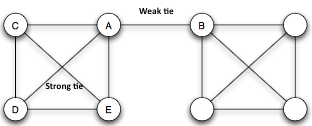
\includegraphics[width=0.95\textwidth]{weakStrongTies.png}
\end{center}
\caption{Weak vs. Strong ties: edge A-B is a weak tie while edge C-E is a strong tie}
\label{fig:figA}
\end{figure}

\textbf{Graph Generation Models} Historically, three different graph models have been studied: 
\begin{enumerate}
\item Random graphs: graphs generated by starting with a disconnected set of nodes that are then paired with a uniform probability
\item Watts and Strogatz graph: graphs with small-world properties\footnote{most nodes can be reached from every other node by a small number of steps}, including short average path lengths and high clustering
\item Scale-free networks: graphs characterized by a highly heterogeneous degree distribution, which follows a "power-law"
\item The Barab́asi-Albert model: the first network with a power-law distribution
\end{enumerate}
These graphs are represented as $G = (V, E)$, with $V$ showing the set of Vertices e.g, people and $E$ corresponding to edges e.g., friendship relationship. A path consists of a set of edges connecting two nodes together. There are three important concepts regarding reproduction of complex social network structure: 

\begin{enumerate}
\item Average path length: showing the average value of length of different paths that characterizes a network's compactness.
\item Degree distribution: the probability distribution of degrees over the network
\item Clustering coefficient %which was described above
\end{enumerate}

Random networks, also known as Erdos-Renyi networks, are an entirely random network based on a probability $p$ of connecting nodes. They have short path length and independent edges. %However, ER graphs do not generate local clustering and triadic closure, and their degree distribution converges to a Poission distribution. 
Social networks are not random graphs since they represent preferential attachment and small world behavior. Preferential attachment refers to the observation that in networks that grow over time, the probability that an edge is added to a node with $d$ neighbors is proportional to $d$.  The concept of small-world networks introduced by Watts and Strogatz (WS) characterizes networks in which most nodes can be reached from every other in a small number of steps (following the six degree of separation theory). 
%They began with a nearest-neighbor coupled network but randomly rewired each edge with probability $p$, to create networks with short average path length and high clustering. Both of random and small-world networks are known as exponential networks because of their homogeneous connectivity distribution with peak at average value. 
%They are based on real social networks, and the average path length can drop rapidly under the conditions of having a small probability of rewiring and almost same clustering coefficient as initial value. 

Unlike the last two static structures,  scale-free networks are dynamically formed by continuous addition of new nodes to the network, and don't have uniform probabilities for creation of new edges. The two main ingredients for self-organization of a network in a scale-free structure are growth and preferential attachment. The corresponding degree distribution is a power law. These networks have smaller average path length compared to random graphs and small-world networks \cite{wangStructure}. %with the same size and same average degree
\citet{barabasi}  introduced an algorithm for generating a network with power-law distribution and having two ingredients of growth and preferential attachment. Growth is the concept regarding the observation that most real-world networks describe open systems that grow by the continuous addition of new nodes.
An important corollary of graph structures is introduced below.

%Now, it is also important to mention another concept introduced in social networks that was used in some of the research explained in use cases.

\textbf{Friendship Paradox} The concept of friendship paradox is derived from graph generation models and their properties. \citet{feld} introduced the concept of friendship paradox. Using general mathematical properties of social networks, he showed that on average most people have fewer friends than their friends have and he called this the "Friendship Paradox". This phenomenon was explained as a consequence of the general mathematical properties of social networks. Assuming the graph of social network $G = (V, E)$ with $V$ showing the set of people and $E$ corresponding to friendship relationship. He modeled the average number of friends of a person in the social network as the average of the degrees of people in the graph. And the average number of friends that a typical friend has, was modeled by choosing uniformly at random an edge and an endpoint of that edge, followed by calculating the degree of the selected endpoint again. \citeauthor{feld} formally proved that your friends have more friends than you do in \cite{feld}.

This implies that friends of a randomly selected person are likely to have higher than average centrality which is an important concept in various applications such as in the case of epidemics and outbreak detection as discussed in \ref{FP}.
% It is obvious that average number of friends of a typical friend is greater than average number of friends of a person, since $\mu$ and $\phi^2$ (the variance) are positive. This proves this theorem which was used in some research explained in use cases.
%\begin{equation}
%\label{teq1}
%\mu = \frac{\sum_{v\in V}d(v)^2)}{\left | V \right |} = \frac{2\left | E \right |}{V}
%\end{equation}
%\begin{equation}
%\label{teq2}
%\frac{\sum_{v\in V}d(v)^2)}{2\left | E \right |} = \mu + \frac{\phi ^ 2}{\mu}
%\end{equation}

\subsubsection{Information Diffusion and Cascades}
%concept of diffusion in social networks? The relation to social sensors? News, opinions, rumors, fads, urban legends, viral marketing, 
In this section, we provide studies on how social network structures support the diffusion of information. It will be shown that the topology of a network has great influence on the overall behavior of information cascades and pattern of epidemic spreading. Information cascade occurs when a person observes the actions of others and then  engages in the same act, even though it can be in contradiction with his/her own private information. %citet{mitra} shows that gossip is fundamental in social groups, existed from early times, and a lot of questions can be answered based on that. Morever, they showed that people gossip with their peers and power law distribution exists between frequency of emails and number of recipients. 

\textbf{Diffusion Models} Given a social network and estimates of reciprocal influence, viral marketing a.k.a. the influence maximization problem is defined to target the most influential users in the network in order to activate chain-reaction of influence and eventually influence largest number of users in the network \cite{richardson}. Two basic classes of diffusion models exist: Linear Threshold Model and Independent . These models represent social network as a directed graph with a binary variable for infection associated to each node (person). Each active node may trigger activation of neighboring nodes. 
\begin{enumerate}
\item Linear Threshold Model: each node has random threshold $\theta_{v} \sim  U\begin{bmatrix} 0, 1 \end{bmatrix}$, and is influenced by each neighbor according to some weight. It becomes active if $\theta_{v}$ fraction of its neighbors are active.
\item Independent Cascade Model: if a node becomes active, it has a single chance of activating each currently inactive neighbor for all time. The activation attempt succeeds with a certain probability related to those two nodes.
\end{enumerate}

%a.k.a. homogeneous contact network
\textbf{Epidemic spread} In classic epidemiology individuals have an equal chance of contact . However, this was determined to be unrealistic. In response,\citet{newman} introduced an underlying contact networks model \cite{newman}. Contact network represents each person as a node and contact as edges and the network can change based on the pathogen. Probability of contagion and length of infection is controlled by the contact network structure. A node will become infected if and only if there is a path to the node from one of the initially infected nodes. \cite{pastor}

The terminology for epidemiological models include:
\begin{itemize}
\item S: Susceptibles
\item E: Exposed individuals in the latent period
\item I: Infectives
\item R: Recovered with immunity
\item $\beta$: Contact rate
\end{itemize}
The three variables $S(t)$, $E(t)$, $R(t)$, $I(t)$ represent the number of individuals with the specified state at the time $t$ and $\beta$ is a real valued variable showing the contact rate or the probability of contagion after contact per unit of time.
Famous epidemiological models include:
\begin{enumerate}
\item SI: Susceptible-Infected \cite{newman}
\item SIR: Susceptible-Infected-Removed \cite{kermack}
\item SIS: Susceptible-Infected-Susceptible
\item SEIR: Susceptible-Exposed-Infected-Removed 
\end{enumerate}
These models show potential stages individuals would go through and they model number of individuals in each stage as random variables. In general, patterns of epidemic spread depend on a disease's contagiousness $\beta$.

In homogeneous networks where individuals have $k$ possibilities of getting the contagion from neighbors, growth of epidemics depends on $\beta$  and $k$ and therefore depends on an epidemic threshold. Different from that, scale-free networks have a different equation for all nodes of same degree $k$, instead of assuming homogeneous mixing. Nodes with higher degrees are more susceptible to infection. Finally, we can observe that there is no epidemic threshold for (infinite) scale-free networks. In practice, the epidemic threshold in scale-free networks is going to be very small and finite-sized scale-free networks are susceptible to epidemic spread regardless of spreading rate.

Similar to this, social contagion phenomena refer to various processes that depend on the individual propensity to adopt and diffuse knowledge, ideas, information. Similar to epidemiological models:
\begin{itemize}
\item Susceptible: an individual who has not learned new information
\item Infected: the spreader of the information
\item Recovered: aware of information, but no longer spreading it
\end{itemize}
Two main questions are: 1) if the rumor reaches high number of individuals i.e. go viral, 2) rate of infection spread
	
\section{Conclusions and Discussion of Open Areas}
% e.g., Learn Tunable Sensors for Specific Tasks, Co-training/Learning error rates of independent sensors on large unlabeled data
% open area: learning to weight items, consider temporal relevance

In conclusion, through review of the literature we showed that social media can be used as a sensor to detect latent phenomena. These works successfully detected or predicted events, sentiments, and preferences of users. The analysis of various works for each use case leveraged various research subfields of analysis of social media.

Results showed that different methods can be successfully applied for each task. For example, classification, regression, clustering, and collaborative filtering methods provided satisfactory results for tasks of sentiment analysis, event detection, and preferences.
% classification methods using lexicon features would provide satisfactory results on sentiment analysis systems. In contrast, monitoring the post rate of events using statistical methods is the way for detecting events.

However, it was shown that the results of some other tasks such as detection of political preferences had low accuracies. One of the reasons is poor generalization from social media user's opinions to the whole country's opinion. As an example, in a big country such as U.S., lot's of middle age or older people don't use social media networks for expressing their opinion. For example, only $23%$ of online adults use Twitter while $71%$ of online adults use Facebook \cite{PewResearchCenter}. This shows the need for more detailed research into 
In general, there is still a gap in detection of these phenomena from social media. The survey results indicate that there is a lack of smart methods for selecting user and learning better sensors compared to existing basic and off-the-shelf classifiers.

Therefore, future expansions of this area includes:
\begin{itemize}
\item Learning tunable sensors for each specific task such as detection of events, trending topics, disasters, epidemic, sentiment, and preference. A large body of work in detection of these tasks define use of sensors, but rely on ad-hoc methods based on data mining or simple statistics to select sensors. In contrast, we intend to learn tunable sensors for each task.
\item Investigate the inclusion of temporal relevance in sentiment analysis methods. People tend to change their emotion and feeling toward topics over time. However, no one has yet to model the dynamics of opinion. We will focus on considering temporal dimension of data in our work.
\item Co-training/learning error rates of independent sensors on large unlabeled data \cite{platanios, blum}. This would enable us to take advantage of semi-supervised learning and, in turn, use all data including unlabeled data. %In addition, it would help in recognition of limiting error-rates
\end{itemize}

Finally, we establish a current state of practice in use of social media as a sensor. We discussed the theories supporting this concept and their abilities to answer the questions of how we can detect latent phenomena in real-time and what features of social networks and text allow us to do so. We surveyed use cases covering the use of social media to detect trending topics, natural disasters, health epidemics, sentiments, preferences, and individual traits. What remains is the need for thorough research into learning tunable sensors, the dynamics of user's opinion, and the learning error rates of independent sensors.

\bibliographystyle{plainnat} 
\bibliography{mybib.bib}

%\bibliographystyle{unsrt} 
%\bibliography{Social Media Sensors}

\end{document}